\documentclass[12pt]{article}
% add some essential packages, some might not be used

\usepackage[T1]{fontenc}
\usepackage[utf8]{inputenc}
\usepackage[usenames,dvipsnames]{color}
\usepackage{natbib}
\usepackage{authblk}
\usepackage{ragged2e}
\usepackage{amsmath}
\usepackage[a4paper,margin=1in,bottom=1.0in]{geometry}
\usepackage{url}
\usepackage{array}
\usepackage{bbding}
\usepackage{amssymb}
\usepackage{graphicx}  % mini page function
\usepackage{adjustbox}
\usepackage{subcaption}
\usepackage{booktabs}
\usepackage{float}
\usepackage{appendix} % appendix package
\usepackage{hyperref}
\usepackage{url}
\usepackage[english]{babel}
\usepackage{adjustbox}
\usepackage{enumitem}
\usepackage{textgreek}
\usepackage{bibentry}
\nobibliography*
\usepackage{lipsum}


\usepackage{listings}
\usepackage{wasysym}
\usepackage{amsthm}
\usepackage{framed}
\usepackage{bm}
\usepackage{booktabs}  % package for table line
% \usepackage{amsrefs?}  % ams citation style package


\usepackage{rotating} % for the horizontal page table

\usepackage{tikz}
\usetikzlibrary{calc}
\usetikzlibrary{matrix}
\usetikzlibrary{positioning}
\usepackage{color}
\usepackage{setspace}
\usepackage{xcolor}

\usepackage{tcolorbox} % package for making colorful box

 \setlength{\parskip}{0.15cm} % change the paragraph spacing
\renewcommand\labelitemi{$\vcenter{\hbox{\tiny$\bullet$}}$} % set the bullet size as tiny

% \newcommand*\rot{\rotatebox{90}} % for rotate text

\usepackage{sectsty} %package for section size

\sectionfont{\fontsize{14}{12}\selectfont} % Change the section font size

\subsectionfont{\fontsize{13}{12}\selectfont}
\subsubsectionfont{\fontsize{12}{12}\selectfont}

\newcommand\numberthis{\addtocounter{equation}{1}\tag{\theequation}} % new command



\theoremstyle{definition}
\newtheorem{definition}[subsection]{Definition}
\newtheorem{axiom}[subsection]{Axiom}
\newtheorem{example}[subsubsection]{Example}
\newtheorem{theorem}[subsection]{Theorem}
\newtheorem{proposition}[subsection]{Proposition}
\newtheorem{lemma}[subsection]{Lemma}


\usepackage{courier}

% tikzsetting

\usetikzlibrary{shapes,decorations,arrows,calc,arrows.meta,fit,positioning}

\tikzset{
    -Latex,auto,node distance =1 cm and 1 cm,semithick,
    state/.style ={ellipse, draw, minimum width = 0.7 cm},
    point/.style = {circle, draw, inner sep=0.04cm,fill,node contents={}},
    bidirected/.style={Latex-Latex,dashed},
    el/.style = {inner sep=2pt, align=left, sloped}
}

\lstset{language=Python}

\definecolor{mygreen}{rgb}{0,0.6,0}
\definecolor{mygray}{RGB}{145, 153, 165}
\definecolor{mymauve}{rgb}{0.58,0,0.82}

\lstset{
  backgroundcolor=\color{white},   % choose the background color; you must add \usepackage{color} or \usepackage{xcolor}; should come as last argument
  basicstyle=\footnotesize,        % the size of the fonts that are used for the code
  breakatwhitespace=false,         % sets if automatic breaks should only happen at whitespace
  breaklines=true,                 % sets automatic line breaking
  captionpos=b,                    % sets the caption-position to bottom
  commentstyle=\color{gray},    % comment style
  deletekeywords={...},            % if you want to delete keywords from the given language
  escapeinside={\%*}{*)},          % if you want to add LaTeX within your code
  extendedchars=true,              % lets you use non-ASCII characters; for 8-bits encodings only, does not work with UTF-8
  frame=single,	                   % adds a frame around the code
  keepspaces=true,                 % keeps spaces in text, useful for keeping indentation of code (possibly needs columns=flexible)
  keywordstyle=\color{RoyalBlue},       % keyword style
  language=Python,                 % the language of the code
  morekeywords={*,...},            % if you want to add more keywords to the set
  numbers=left,                    % where to put the line-numbers; possible values are (none, left, right)
  numbersep=5pt,                   % how far the line-numbers are from the code
  numberstyle=\tiny\color{gray}, % the style that is used for the line-numbers
  rulecolor=\color{black},         % if not set, the frame-color may be changed on line-breaks within not-black text (e.g. comments (green here))
  showspaces=false,                % show spaces everywhere adding particular underscores; it overrides 'showstringspaces'
  showstringspaces=false,          % underline spaces within strings only
  showtabs=false,                  % show tabs within strings adding particular underscores
  stepnumber=2,                    % the step between two line-numbers. If it's 1, each line will be numbered
  stringstyle=\color{mymauve},     % string literal style
  tabsize=2,	                   % sets default tabsize to 2 spaces
  title=\lstname                   % show the filename of files included with \lstinputlisting; also try caption instead of title
}

\numberwithin{equation}{section}
\numberwithin{figure}{section}
\numberwithin{table}{section}


% Define colors
\definecolor{cmd}{HTML}{F7F7F9}
\DeclareMathOperator{\di}{d\!}

\newcommand{\pr}{$\mathbb{P}$}
\newcommand{\pre}{\mathbb{P}}

\begin{document}

\title{Classification: Logistic Regression and Linear Discriminant Analysis}
\author{Michael}
\date{}
\maketitle


\section{Intuition Behind Logistic Regression}

In statistics 101 or econometrics 101, students are taught that they should be aware of the properties of independent variables. For instance, when we want to study the effects of different factors, such as education, gender, family background, etc., on individual's income level, we have to know that gender is dummy variable, education is categorical variables, etc. We don't care too much whether independent variables are continuous or not (e.g., dummy variable is not continuous) as long as dependent variable ($Y$) is continuous. Why? Because we need $Y$ is continuous when we want to do differentiation to find the optimal solutions.

What if dependent variable $Y$ now becomes discrete values, such as 1, 2, 3, 4, which they are not continuous? We need employ the logistic transformation to bring the model into a continuous domain. Through the logistic transformation, we \textit{link our categorical values(like class A, B, C) with certain probability values ($\pi \in [0, 1]$)}.


Now, we would like to have the probability $\pi_i$ depend on a vector of observed covariates $x_i$ (e.g., education, income). The simplest idea would be to let $\pi_i$ be a linear function of the covariates, say
\begin{equation}
	\pi_i = x_i'\beta
\end{equation}
where $\beta$ is a vector of regression coefficients. This model sometimes is also called the linear probability model. Once we get the estimated probability $\hat{\pi}$, if we can compare it with benchmark value, say if $\hat{\pi} > 0.6$ then observation with $x_i$ characters can be classified as class A.

However, one problem with this model is that probability $\pi_i$ on the left hand side has to be between 0 and 1, but the linear predictor $x_i'\beta$ on the right hand side can take any real value, so there is no guarantee that the predicted values will be in the correct range unless complex restrictions are imposed on the coefficients.

A simple solution to this problem is to transform the probability to remove the range restrictions, and model the transformation as a linear function of the covariates. We do this in two steps:
\begin{enumerate}
	\item  we move from the probability $\pi$ to the odds: $$odds_i = \frac{\pi_i}{1-\pi_i}$$
	\item we take logarithms, calculating the $logit$ or log-odds: $$\eta_i = \log(odds) = \log (\frac{\pi_i}{1-\pi_i}), where \ \eta \in (-\infty, + \infty)$$
\end{enumerate}

Now, Now, let's do some simple algebra and begin to use MLE. Solving for $\pi_i$ in above equation, it gives
\begin{equation}
	\pi_i = logit^{-1}(\eta_i) = \frac{e^{\eta_i}}{1+e^{\eta_i}}
\end{equation}

We are now in a position to define the logistic regression model, by assuming that the logit of the odds ratio, rather than the probability itself, follows a linear model:
\begin{equation}
	log(\frac{\pi_i}{1-\pi_i}) = x_i' \beta \ \ \Rightarrow \frac{\pi_i}{1-\pi_i} = e^{x_i'\beta} \ \ \Rightarrow \pi_i = F(x_i'\beta) = \frac{e^{x_i'\beta}}{1+e^{x_i'\beta}}
\end{equation}

In this case marginal effect can be obtained as
\begin{equation}
	\frac{d\pi_i}{dx_{ij}} = \Big[ \frac{e^{x_i'\beta}}{(1+e^{x_i'\beta})^2} \Big]\beta_j = [\frac{e^{x_i'\beta }}{(1+e^{x_i'\beta})} \frac{1}{(1+e^{x_i'\beta})} ] \beta_j = \beta_j \pi_i(1-\pi_i)
\end{equation}

\section{Logistic Regression}

Most of content in this section is taken from the notes by \cite{ng2014cs229}. As it has shown in (1.3), we can get a continuous function (or map) between covariates $x$ and dependent variable probability $\pi$:
\begin{align}
  \pi = h_{\theta}(x) = \frac{e^{\theta' x}}{ 1 + e^{\theta' x}} = \frac{1}{1+ e^{-\theta' x}}
\end{align}
where the general format
\begin{align*}
  g(z) = \frac{1}{1+e^{-z}}
\end{align*}
is called the \textbf{logistic function}.

So, given the logistic regression model, how do we fit $\theta$ for it? As we are using the probability now, we need employ the maximum likelihood. Let us assume that
\begin{align*}
  P(y = 1 | x; \theta) & = h_{\theta}(x) \\
  P(y = 0 |x; \theta) & = 1 - h_{\theta}(x)
\end{align*}
Note this can be written more compactly as
\begin{align}
  P(y |x; \theta) = (h_{\theta}(x))^y (1 - h_{\theta}(x))^{1-y}
\end{align}
Assuming that the m training examples were generated independently, we can then write down the likelihood of the parameters as
\begin{align*}
  L(\theta) & = \prod_{i=1}^m P(y^{i}| x^{i}; \theta) \\
  & = \prod_{i=1}^m (h_{\theta}(x))^y (1 - h_{\theta}(x))^{1-y}
\end{align*}

How do we maximize the likelihood? We can still use gradient descent method. However, as we are doing maximum of likelihood rather than the minimum of cost function, so our update rule will become (we also call descent ascent not descent)
\begin{align*}
  \theta = \theta + \alpha \Delta_{\theta} l (\theta)
\end{align*}
where $\Delta_{\theta} l (\theta)$ is the just derivative of our likelihood function. Now, let's take one training example (x, y) and take derivative:
\begin{align*}
  \frac{\partial L(\theta)}{\partial \theta} & = \bigg(y \frac{1}{g(\theta' x)} - (1 - y) \frac{1}{1 - g(\theta' x)} \bigg) \frac{\partial }{\partial \theta_j} g(\theta' x) \\
  & = (y - h_{\theta}(x)) x_j \\
  & = (y - \frac{1}{1+e^{-\theta' x}})x_j
\end{align*}
This therefore gives us the \textit{stochastic gradient ascent} rule
\begin{align}
  \theta_j = \theta_j + \alpha (y^i - h_\theta(x^i))x_j^i
\end{align}
where
\begin{align*}
   h_{\theta}(x) = \frac{e^{\theta' x}}{ 1 + e^{\theta' x}} = \frac{1}{1+ e^{-\theta' x}}
\end{align*}

If we have more than two categories to classify, we can still use logistic regression to model the classification. However, the method is not as efficient as linear discriminant analysis, which we will go through in the next section.

\section{Intuition Behind Linear Discriminant Analysis}

The famous Bayes' rule is
\begin{align}
	P(A|B) = \frac{P(B|A)P(A)}{P(B)}
\end{align}

Linear discriminant analysis is just built upon the above formula. Please make sure you got the intuition behind this formula. To help us to grasp the intuition of (3.1), we can write it as 
\begin{align*}
	P(A|B)P(B) = P(B|A)P(A)
\end{align*}
This means that the probability of A happens condition on B is same with the probability of B happens condition on A. In words: \textit{The probability of A is girl condition on B (colorful nails, long hairs, etc.) is same with the probability of B (colorful nails, long hairs, etc.) happens conditional on A is a girl}. 

\textbf{Be careful}, we are talking about probability, rather than the absolute case, A can still be a boy with B (colorful nails, long hairs, etc.). But the probability of being girl should be higher, say 0.8. 

Now, suppose $f_k(x)$ is the class-conditional density of $X$ in class $G = k$, and let $\pi_k$ be the prior probability of class k, with $\sum_{k = 1}^K \pi_k = 1$. A simple application of Bayes theorem gives us
\begin{align}
  P(G = k | X = x) = \frac{f_k(x) \pi_k}{\sum_{l = 1}^K f_l(x) \pi_l}
\end{align}

Although (3.2) looks very intimidating, it means the same thing with (3.1), which we can write it as
\begin{align*}
	P(G = k | X = x) = \frac{P(X = x| G = k)P(k)}{P(X = x)}
\end{align*}

But, how do we usually get $P(k)$ or $P(X = x| G = k)$? We either can calculate it with the sample or we can get it through density function\footnote{Review the difference between probability density function (pdf) and cumulative density function (cdf).}. Suppose we know the density function, then we can have 
\begin{align*}
	f_k(x) = P(X = x| G = k)
\end{align*}
Now, we use $\pi_k$ to represent $P(k)$
\begin{align*}
	\pi_k = P(k)
\end{align*}

For $P(x)$, we can decompose it as several cases by employing the conditional probabilities again: 
\begin{align*}
	P(x) = P(X = x|k =1) P(k=1) + P(X = x |k=2) P(k=2) + \cdots + P(X= x|k=K) P(k=K)
\end{align*}


Now, once you understand (3.2), then the following part will be just the manipulation of formulas. Let's restate (3.2) again, to make sure you feel comfortable with it:
\begin{align*}
  P(G = k | X = x) = \frac{f_k(x) \pi_k}{\sum_{l = 1}^K f_l(x) \pi_l}
\end{align*}


\section{Linear Discriminant Analysis}

Question we need answer: what's the value of $Y$ if you give me values of $X$? From now on, we use $Y$ as the dependent value, for example $Y = 0$ means girl, $Y=1$ means boy; and $X$ as the independent values, for instance, a matrix represents the characteristics of boys and girls. 

Now we model $P(X = x | Y = k) = f_k(x)$ as a \textit{multivariate normal distribution}, and we know $P(Y = k) = \pi_k$ exactly. And the multivariate normal distribution with density
\begin{align}
	f_k(x) = \frac{1}{(2\pi)^{m/2}|\Sigma_k|^{1/2}}	e^{-\frac{1}{2} (x - \mu_k)^T \Sigma^{-1}(x - \mu_k) }
\end{align}
where $|\Sigma_k|$ is the determinant of covariance matrix, $m$ is the number of covariate variables. Say $X$ is a $n \times m$ matrix, $n$ is the number of observations, and $m$ is the number of covariate variables (length of hair, colors of nail, etc). In our example, $m$ is equal to two, one for hair, one for colors of nail. 

We are modeling each class $k$ density as multivariate normal distribution. That's why we have $k$ as subscript in (4.1). Now, let's give an example, let $k=0$, which means we take $Y =0$ or girls' characteristic, and modeling them as
\begin{align*}
	f_0(x) = \frac{1}{(2\pi)^{m/2}|\Sigma_0|^{1/2}}	e^{-\frac{1}{2} (x - \mu_0)^T \Sigma^{-1}(x - \mu_0) }
\end{align*}

Now, what is $\mu_0$ then? $\mu_0$ is the mean for class $k=0$ or $Y=0$ or girls. In our example with $m=2$, we have 
\begin{align*}
	\mu_0 = \begin{bmatrix}
		60 \\
		5
	\end{bmatrix} = \begin{bmatrix}
		\text{length of hair}(cm)\\
		\text{colors of nails}
	\end{bmatrix} & & \Sigma_0 = \begin{bmatrix}
		1 & 3 \\
		1.2 & 1
	\end{bmatrix}
\end{align*}

if, we take $k=1$, $Y =1$ or boys' characteristic, and modeling them as
\begin{align*}
	f_1(x) = \frac{1}{(2\pi)^{m/2}|\Sigma_1|^{1/2}}	e^{-\frac{1}{2} (x - \mu_1)^T \Sigma^{-1}(x - \mu_1) }
\end{align*}
Then we should have 
\begin{align*}
	\mu_1 = \begin{bmatrix}
		16 \\
		0
	\end{bmatrix} = \begin{bmatrix}
		\text{length of hair}(cm)\\
		\text{colors of nails}
	\end{bmatrix} & & \Sigma_1 = \begin{bmatrix}
		1 & 1.6 \\
		0.8 & 1
	\end{bmatrix}
\end{align*}

\textit{I never measured the length of my hair}, so don't take it too serious on the above numbers. \textbf{Be careful here}, from now on we assume that category 0 and 1 have different mean but have the same covariance matrix $\Sigma$. It is this assumption that makes the modeling we are discussing right now have linear properties. 

Let's restate what have known at this stage. We assume that $P(X = x|Y =k)$ follows the multivariate normal distribution with density (please be aware of the difference between equation 4.1 and 4.2):
\begin{align}
	f_k(x) = f_k(x) = \frac{1}{(2\pi)^{m/2}|\Sigma|^{1/2}}	e^{-\frac{1}{2} (x - \mu_k)^T \Sigma^{-1}(x - \mu_k) }
\end{align}
where $\mu_k$ is the mean of covariate variable (e.g., length of hair) for category k, and $\Sigma$ is the covariance matrix and is common to all categories. By Bayes rule, the probability of category $k$, given the input $x$ is:
\begin{align*}
	P(Y=k|X = x) & = \frac{P(X =x| Y = k) P(Y=k)}{P(X=x)} \\
	& = \frac{f_k(x) \pi_k}{P(X = x)}
\end{align*}
The denominator $P(X=x)$ does not depend on the response $k$, so can use a constant to represent it:
\begin{align*}
	P(Y=k |X = x) = \frac{1}{Constant} f_k(x) \pi_k
\end{align*}
The question we need answer is: what's the value of $Y$ if you give me values of $X$? Hence, we don't need bother to care too much on the constant value. Now, substitute the $f_k(x)$ into the above function, we can have
\begin{align*}
	P(Y=k |X = x) = \frac{1}{Constant} \frac{\pi_k }{(2\pi)^{m/2}|\Sigma|^{1/2}}	e^{-\frac{1}{2} (x - \mu_k)^T \Sigma^{-1}(x - \mu_k) }
\end{align*}

Now, we use the same tricky that absorb everything does not depend on $k$ into a constant $C$:
\begin{align*}
	P(Y=k |X = x) = C \pi_k e^{-\frac{1}{2} (x - \mu_k)^T \Sigma^{-1}(x - \mu_k) }
\end{align*}
Then, we take the logarithm of both sides:
\begin{align}
	\log P(Y=k |X = x) = \log C + \log \pi_k -\frac{1}{2} (x - \mu_k)^T \Sigma^{-1}(x - \mu_k)
\end{align}

Now, it's the time to answer our question: we want to find the maximum of (4.3) over different categories $k$, or in other words, we want to find values of $x$ that can maximize $P(Y=k|X =x)$ if know $\mu_k$ and $\Sigma$. Intuitively, I want to classify $X=x$ that can maximize the probability of $P(Y=0)$ or $P(Y=1)$. Here is the place that LDA algorithm of machine learning kicks in, where you (future data scientist) can tell me whether the future observations (only know $X$, but not $Y$) should be classified as boys/girls or good/bad wines (predicted $Y$). 

Again, we have to the process of maximization, and we will leave the constant $\log C$ as it won't affect the results. Therefore, we need maximize the following over $k$ (the last two parts of equation 4.3): 
\begin{align*}
	 & \log \pi_k -\frac{1}{2} (x - \mu_k)^T \Sigma^{-1}(x - \mu_k) \\
	= &  \log \pi_k - \frac{1}{2}[ x^T \Sigma^{-1} x + \mu_k^T \Sigma^{-1} \mu_k] + x^T \Sigma^{-1} \mu_k \tag{do expansion} \\
	= & - \frac{1}{2}  x^T \Sigma^{-1} x + \log \pi_k - \frac{1}{2} \mu_k^T \Sigma^{-1} \mu_k + x^T \Sigma^{-1} \mu_k \tag{rearrange}
\end{align*}
We do rearrangement to delete the constant value $- \frac{1}{2}  x^T \Sigma^{-1} x $ again, and now we define the objective function without the constant values:
\begin{align}
 \delta_k(x) = 	\log \pi_k - \frac{1}{2} \mu_k^T \Sigma^{-1} \mu_k + x^T \Sigma^{-1} \mu_k 
\end{align}
This is the function we have in p.31 of our lecture sides. At an input $x$, we predict the response with the highest $\delta_k(x)$ as it gives us the highest conditional probabilities: tell me the value of length of hair or number of colored nails, I can tell you $Y$ is a boy or girl. But how? We need boundary value to make decision of being a boy or girl as $\delta_k(x)$ only gives us the probability. I don't want you tell me that 80\% of chance that people with $X$ characteristics (no colored nails) is a boy. I want to the classification (boy or girl, to be or not to be, you tell me) rather than probability. 

\textit{But, wait a minute, how can we maximize equation (4.4) without knowing} $\pi_k$, $\mu_k$ and $\Sigma$? Aha, we have the training data. We use our training data to calculate:
\begin{itemize}
	\item $\hat{\pi_k} = N_k/N$, where $N_k$ is the number of class-k observations, and $N$ is the total number of observations
	\item $\hat{\mu_k} = \sum_{i=k} x_i/N_k$
	\item $\hat{\Sigma} = \sum_{k=1}^K \sum_{i=k} (x_i - \hat{\mu_k})(x_i - \hat{\mu}_k)^T/(N-K)$
\end{itemize}

Figure 4.1 gives the big picture on classification. Now, you should understand why we have a feature function and fit function for LDA classifications. 
\begin{figure}[H]
	\centering
	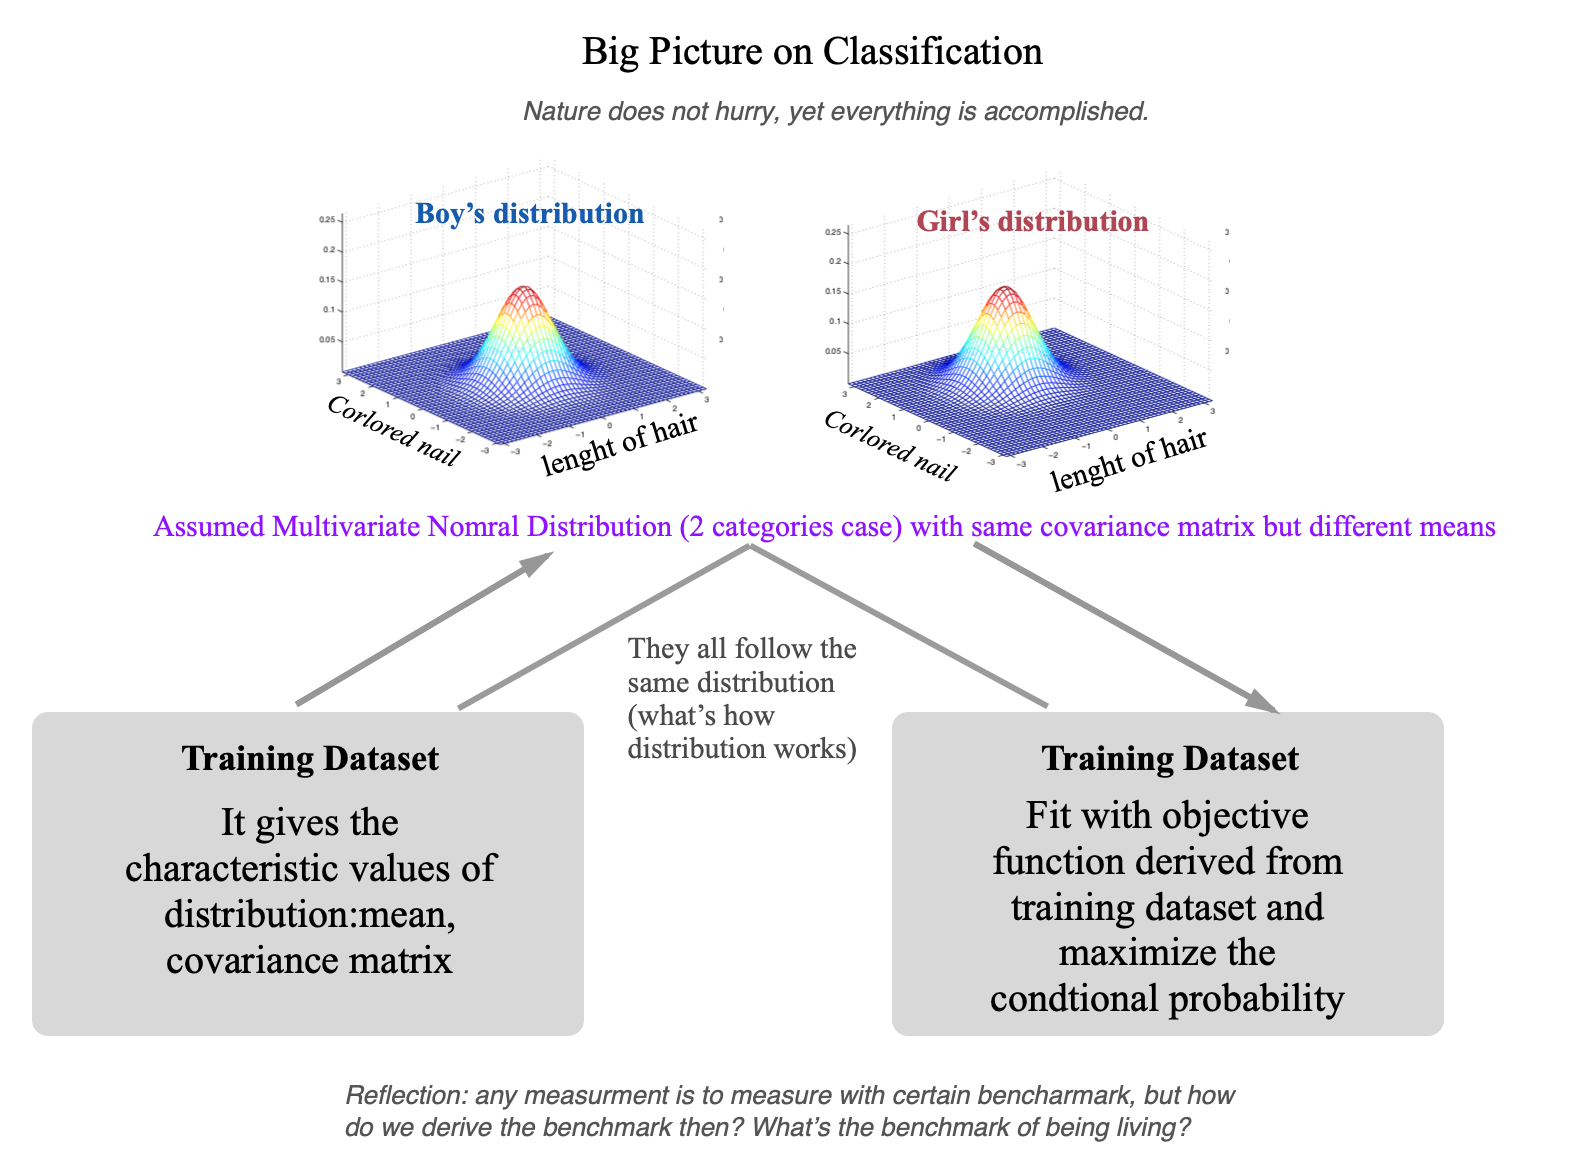
\includegraphics[width=\textwidth]{bigpicture}
	\caption{A picture is worth a thousand words}
\end{figure}

\subsection{The boundary decision and the critical values}

To make the final decision on classification we need have the boundary for our probabilities. Of course we can set a certain number say $0.8$ as a boundary values, which implies that if $\delta_0(x) \geq 0.8$ we can make decision that the observation is a girl. But how about $\delta_1(x)$, should we also use $0.8$ or not? The fair one is the set of points in which 2 classes do just as well or when they are both maximized at the same time:
\begin{align}
	\delta_0(x) & = \delta_1(x) \\
	\log \pi_0 - \frac{1}{2} \mu_0^T \Sigma^{-1} \mu_0 + x^T \Sigma^{-1} \mu_0 & = \log \pi_1 - \frac{1}{2} \mu_1^T \Sigma^{-1} \mu_1 + x^T \Sigma^{-1} \mu_1
\end{align}
Solve (4.6) gives us the critical values of of $x$, which is
\begin{align}
 x_{crit}^T = \frac{1}{(\Sigma^{-1}\mu_1 - \Sigma^{-1}\mu_0)}\big (\log \frac{\pi_0}{\pi_1} + \frac{ \mu_1^T \Sigma^{-1} \mu_1 -  \mu_0^T \Sigma^{-1}}{2} \mu_0 \big )	
\end{align}

This gives a vector that contains all critical values of $x$. In our model, we assume the number of covariates variates is $m$ (see 4.2), so we should get $m$ critical values in the end. Equation (4.7) is in matrix format, where $\mu_1$, $\mu_0$ are vectors of mean values for all covariate variables. We can also calculate the mean and variance for each variable in $X$, say the length of hair, then get the critical value for each covariate variable like the formula we been given in p.33 of our lecture slides:
\begin{align*}
	x_{crit} & = \frac{\sigma^2}{\mu_1 - \mu_0} \big( \log \frac{\pi_0}{\pi_1} + \frac{\mu_1^2 - \mu_0^2}{2 \sigma^2} \big ) \\
	& = \frac{\sigma^2}{\mu_1 - \mu_0} \big( \log \frac{1-\pi_1}{\pi_1} + \frac{\mu_1^2 - \mu_0^2}{2 \sigma^2} \big )
\end{align*}

What if we have more than 2 categories, where $Y=0, 1, 3, 4, \cdots K$, how can we find the critical values of $x_{crit}$? With multi-categories, we need solve a system of linear equations:
\begin{align*}
	\delta_{0}(x) & = \delta_{1}(x) \\
	\delta_{0}(x) & = \delta_{1}(x)  \\
	& \vdots \\
	\delta_{k-1}(x) & = \delta_{K}(x) \\
	\delta_{0}(x) & = \delta_{1}(x) = \cdots = \delta_{K}(x)
\end{align*}
We have $K$ equations for solving $K$ unknowns ($X_{crit}$). It guarantees the solution. 

We will have a case study for $K=3$ categories to understand LDA deeply in later section. 

\section{Quadratic Discriminant Analysis}

The idea and logic for quadratic discriminant analysis (QDA) is same with LDA except for the assumption related to the covariance matrix part. In QDA, we not just estimate $\mu_k$, but also the covariance $\Sigma_k$ for each class separately. This means we do not assume the exist of common covariance matrix $\Sigma$.

Given an input and following the same procedure in LDA, it is easy to derive an objective function:
\begin{align}
	\delta_k(x) = \log \pi_k - \frac{1}{2} \mu_k^T \Sigma_{k}^{-1} \mu_k + x^t \Sigma_{k}^{-1} \mu_k - \frac{1}{2} x^T \Sigma_{k}^{-1}x - \frac{1}{2} \log |\Sigma_{k} |
\end{align}

The objective function is now quadratic in $x$ and so are the decision boundaries. Compare (5.1) with (4.4), you should realize the difference of $x$, one is linear and one is quadratic. 


\section{Final Comment}

LDA and QDA are very powerful tools for classification. It is very often that these two methods are always in the top range in terms of performance compared to whatever exotic tools people invented for doing classifications. 

So, make sure you understand them well. Further readings can be found in the book by \cite{friedman2001elements}. 


\section{Case Study}












\bibliography{/Users/Michael/Documents/MachineLearning/ML.bib}
\bibliographystyle{apalike}
\end{document}
